\chapter [Plot operations in Scilab]{Plot operations in Scilab}


\section*{Problem Definition}
It often requires to visualize the data for clarity in perception. The plot may be continuous or discrete. It may be two dimensional or three dimensional. The requirement is to familiarize plotting capabilities of Scilab.

\section*{Background Details}
\paragraph{}

Scilab is an open source software for numerical mathematics and scientific visualization. We will see the use of \texttt{plot}, \texttt{plot2d}, \texttt{plot2d3}, \texttt{plot3d}, \texttt{surf},  and \texttt{radialplot}

\section*{Let us experiment}

\paragraph{}
\begin{enumerate}
\item
Start Scilab on PC and Scilab console window opens. Create a new blank SciNote.
\item
The code for the required program is typed and saved as Scilab SCE file with an extension .sci

\item

The continuous plots are made using the function “plot” and discrete plots are made using the function “plot2d3” with the corresponding x axis and y axis variables written inside paranthesis.


\item
The results and the errors in the program are displayed in the console window.
The typed program is run using the “execute”.
\end{enumerate}

\section*{Scilab Code and Resulting Plots}
\subsection*{2D plotting}


\lstinputlisting[caption=2D plotting functions]{./scilabCode/plotOperations2d.sci}

The plotted figures are shown in \ref{plot}, \ref{plot2d}, \ref{plot2d3}.

\begin{figure}
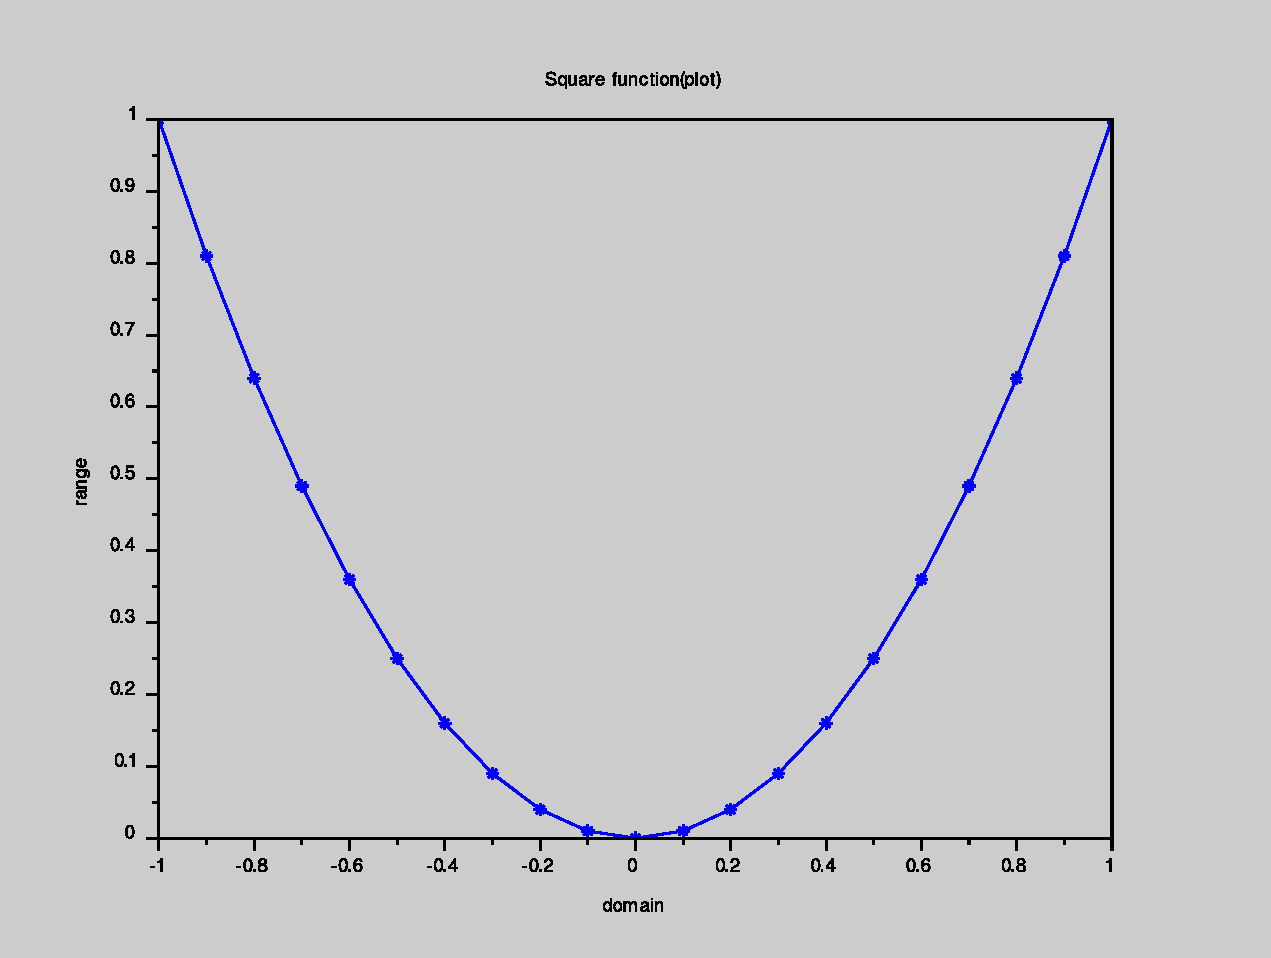
\includegraphics[scale=.5]{scilabCode/plotfunction.pdf}
\caption{Illustrating \texttt{plot} function}
\label{plot}
\end{figure}

\begin{figure}
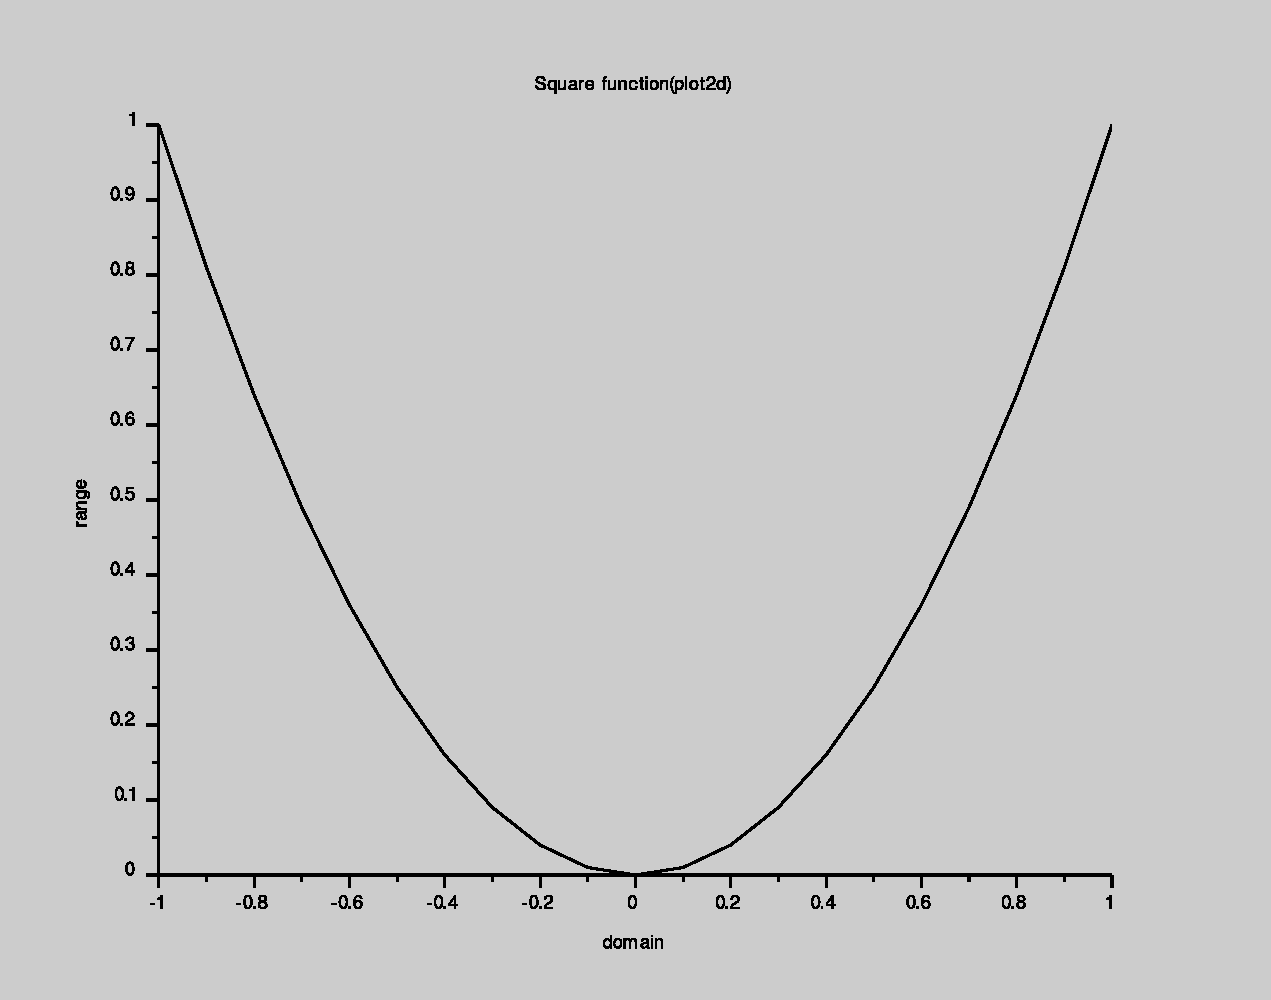
\includegraphics[scale=.5]{scilabCode/plot2dfunction.pdf}
\caption{Illustrating \texttt{plot2d} function}
\label{plot2d}
\end{figure}

\begin{figure}
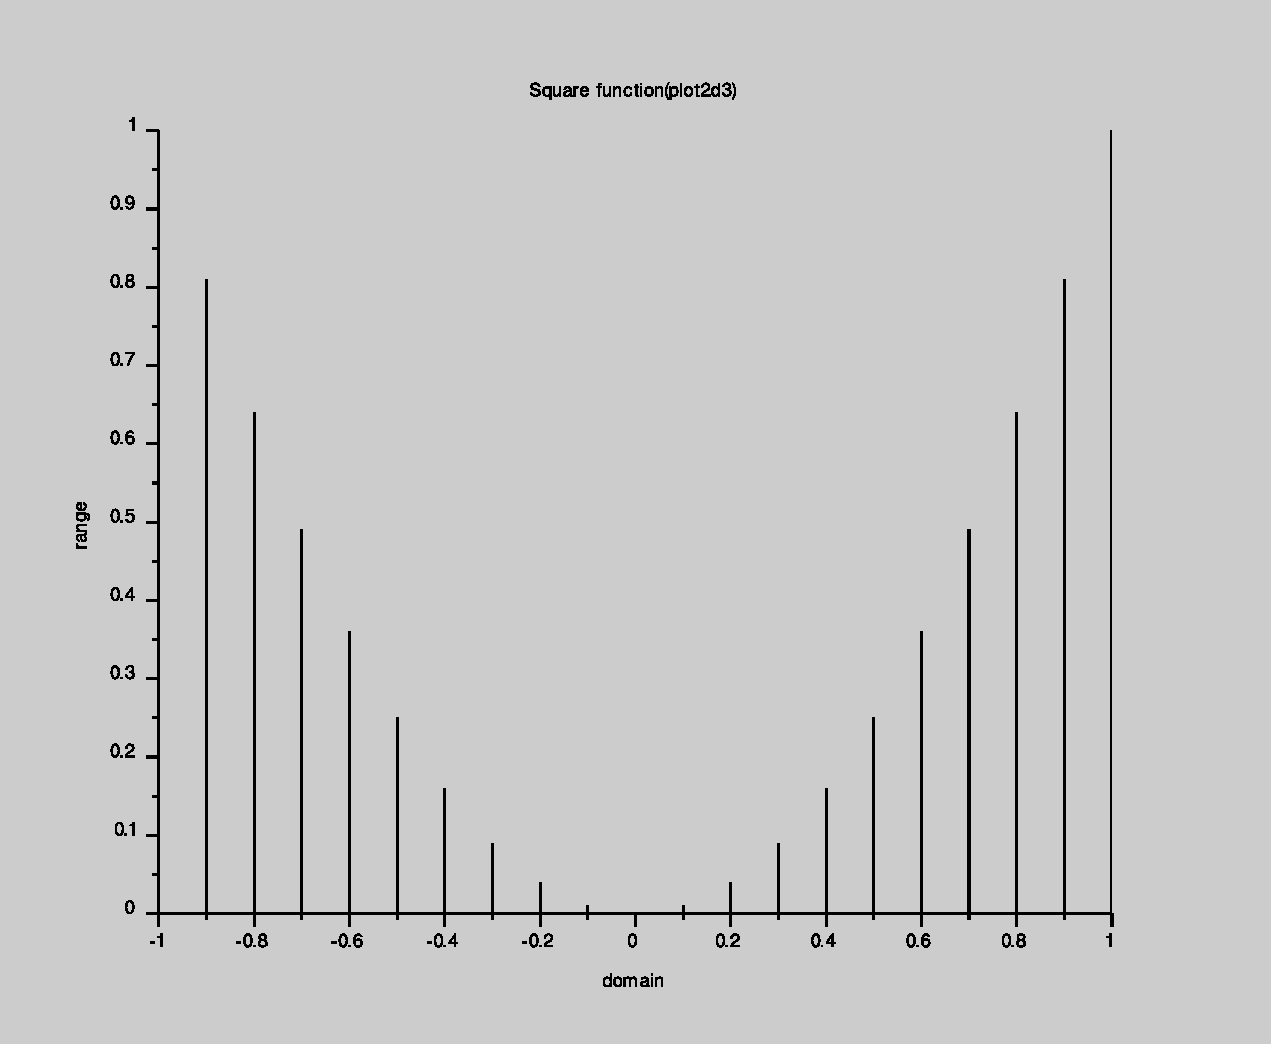
\includegraphics[scale=.5]{scilabCode/plot2d3function.pdf}
\caption{Illustrating \texttt{plot2d3} function}
\label{plot2d3}
\end{figure}

\newpage

\subsection*{3D plotting}
\lstinputlisting[caption=3D Plotting functions]{./scilabCode/plot3d.sci}

The plotted figures are shown in \ref{plot3d},\ref{plot3dsin} and \ref{surf}.

\begin{figure}
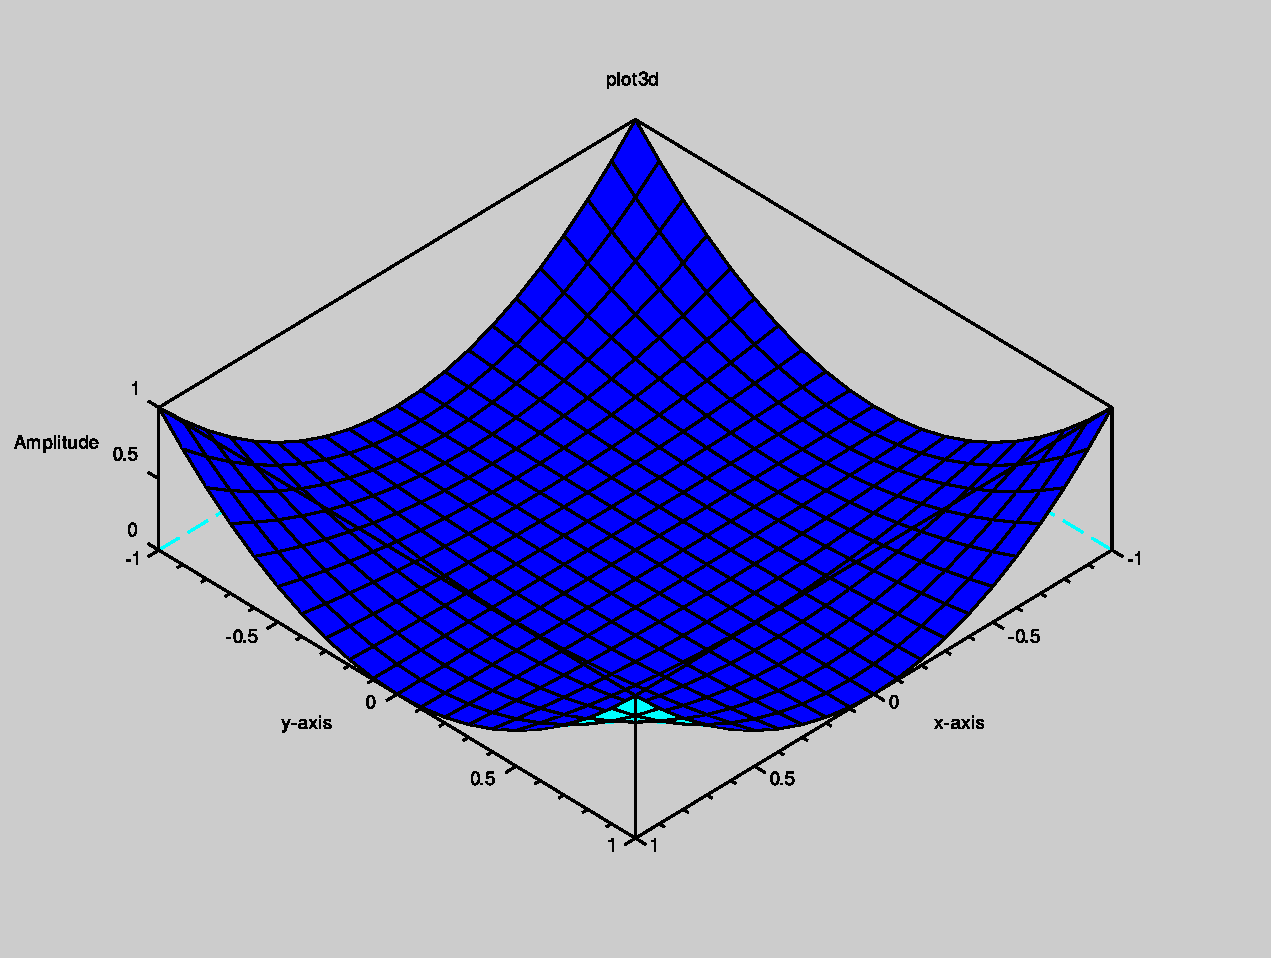
\includegraphics[scale=.5]{scilabCode/plot3d.pdf}
\caption{Illustrating \texttt{plotd3} function}
\label{plot3d}
\end{figure}

\begin{figure}
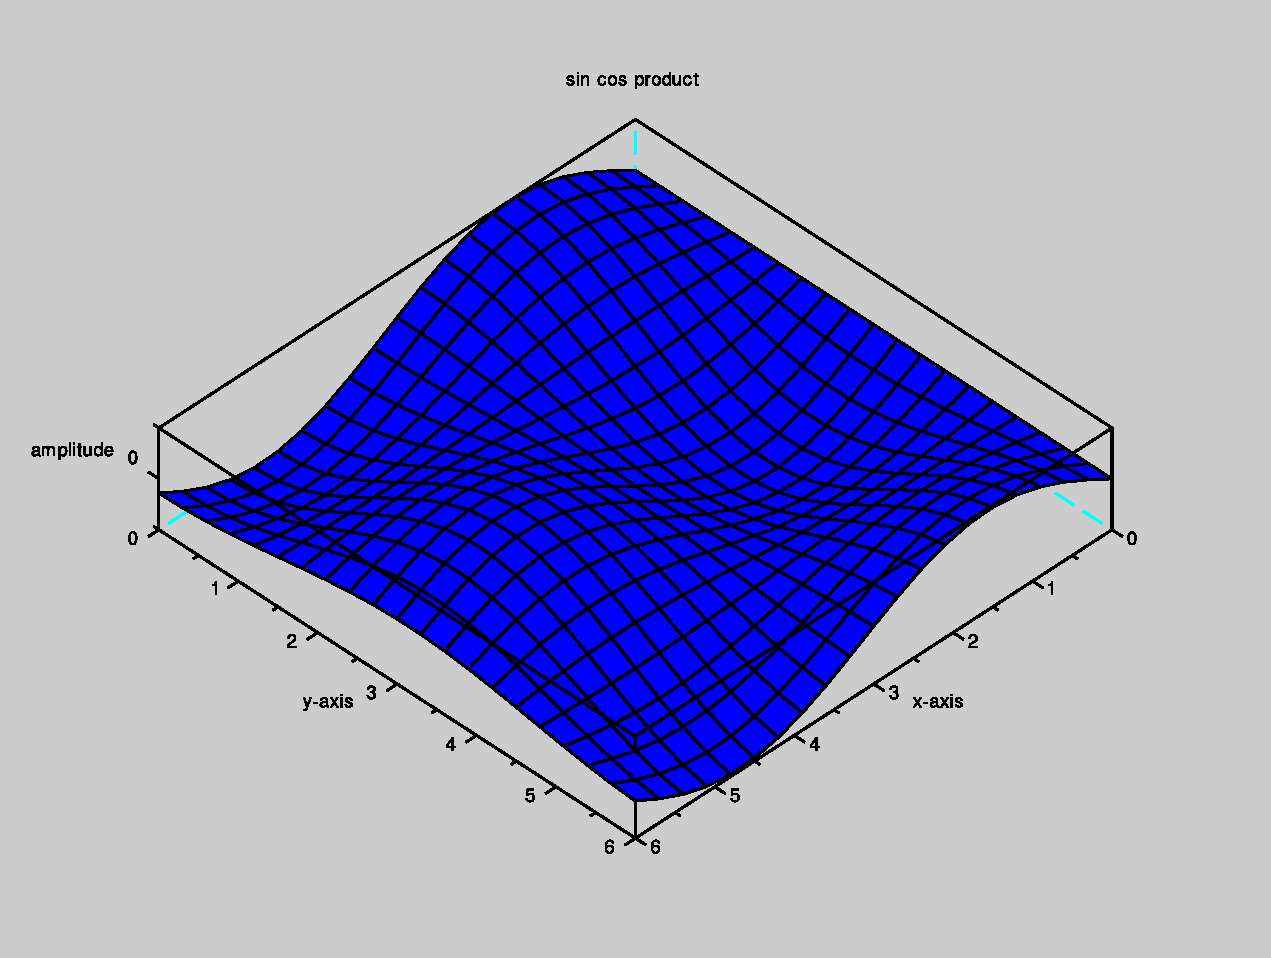
\includegraphics[scale=.5]{scilabCode/plot3dsin.pdf}
\caption{Illustrating \texttt{plot3d} function }
\label{plot3dsin}
\end{figure}

\begin{figure}
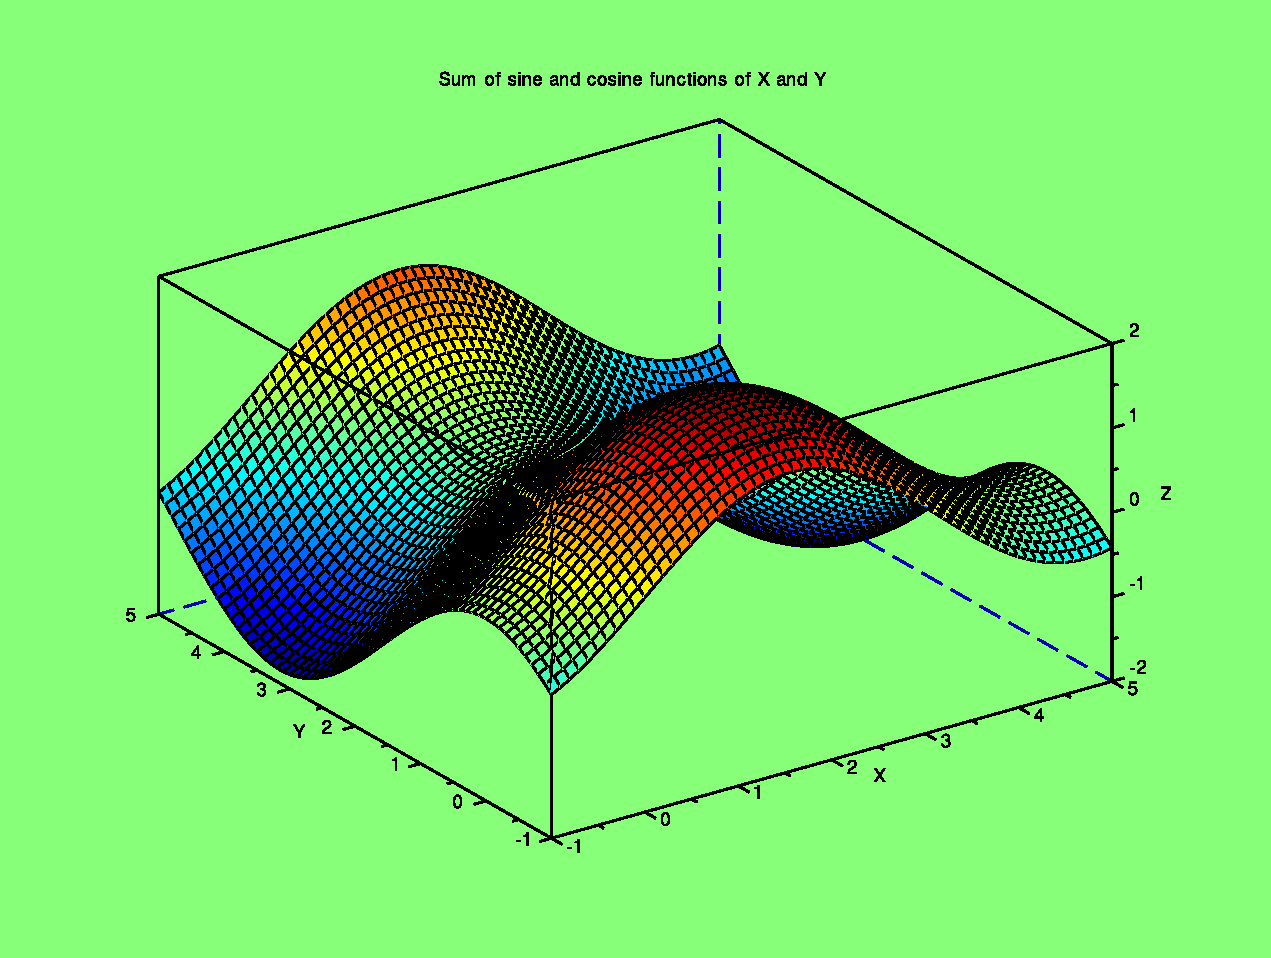
\includegraphics[scale=.5]{scilabCode/surfaceplot.pdf}
\caption{Illustrating \texttt{surf} function}
\label{surf}
\end{figure}
\newpage


\subsection*{Polar plotting}
\lstinputlisting[caption=Polar Plotting functions]{./scilabCode/radialplot.sci}

The plotted figures are shown in \ref{spiral} and \ref{sinSquare}.

\begin{figure}
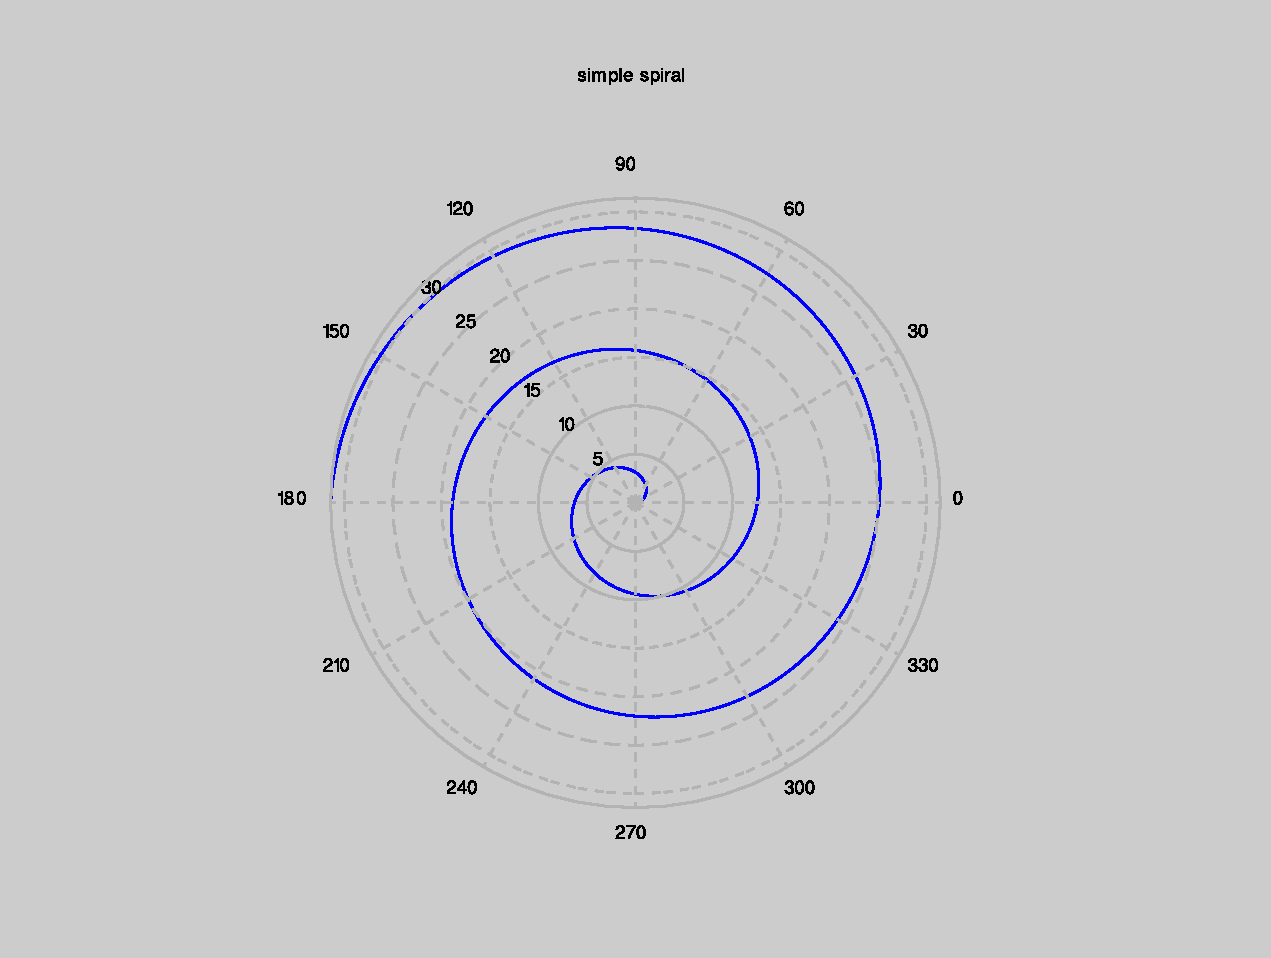
\includegraphics[scale=.5]{scilabCode/spiral.pdf}
\caption{Illustrating \texttt{polarplot} function}
\label{spiral}
\end{figure}

\begin{figure}
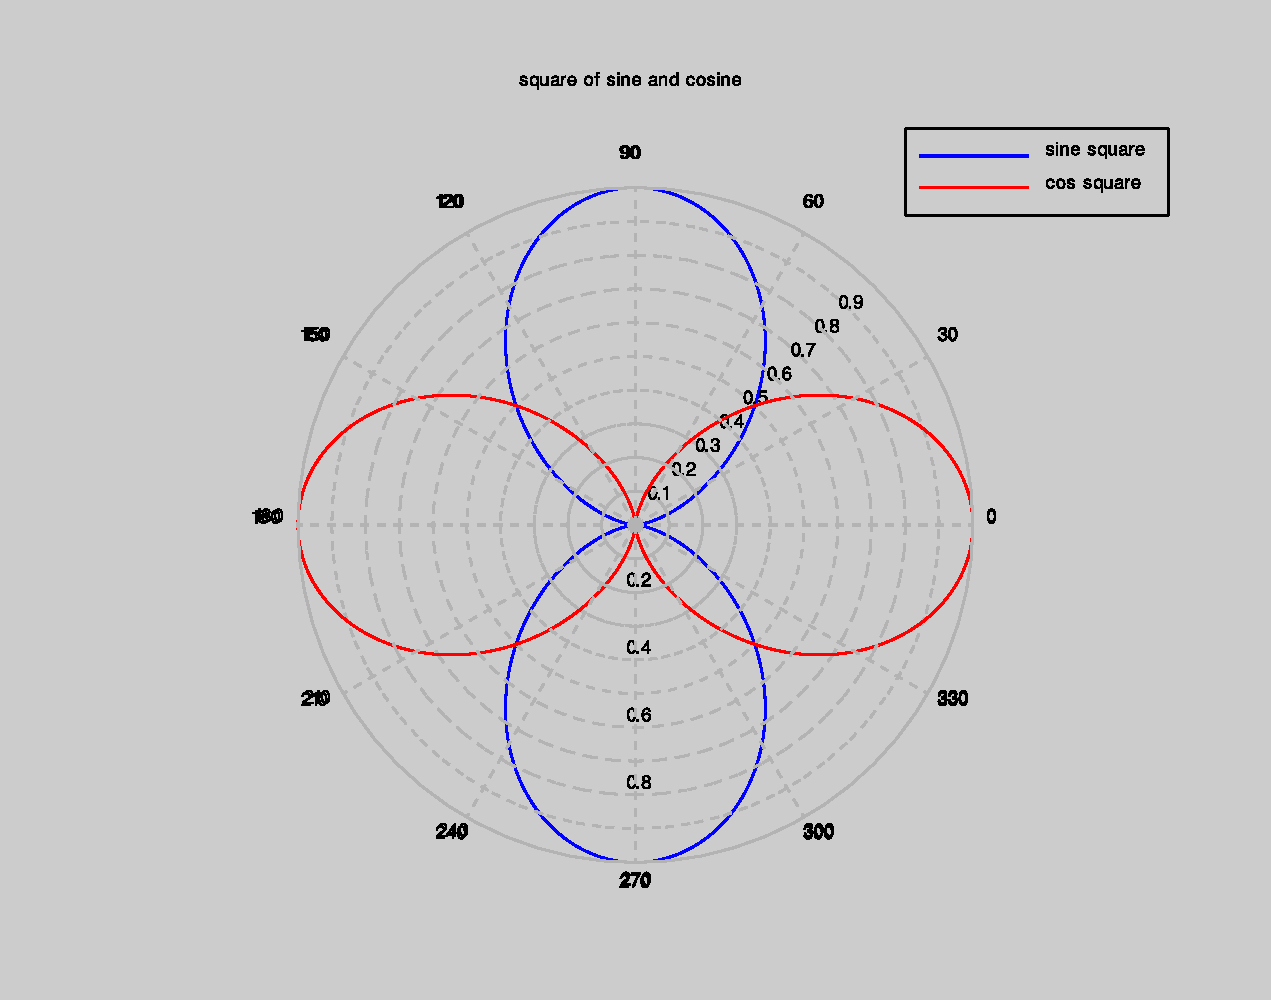
\includegraphics[scale=.5]{scilabCode/sinSquare.pdf}
\caption{Illustrating \texttt{polarplot} function}
\label{sinSquare}
\end{figure}

\section*{Result}

Familairised various plotting capabilities of scilab.
